\subsection{Safety over EtherCAT}

In order to simplify electrical wiring even further, industrial equipment can use the EtherCAT network to distribute safety-critical information regarding its state.
This is a protocol called Safety over EtherCAT (FSoE - Fail safe over EtherCAT), which works by integrating a specialized data frame named Safety Container as if they were generic datagrams inside the standard EtherCAT frame.
This means the safety-critical information is distributed over the network along side the process data, in a cyclic fashion.
This protocol is standardized in IEC 61784-3.

Having this type of safety data transmission allows to more easily expand an existing process with additional hardware or safety features, without having to possibly restructure the entire safety circuit.
Diagnostic functions integrated into the communication mechanism also allow for faster and easier fault detection and correction.

EtherCAT integrates the Safety Containers in a transparent way inside the EtherCAT frame and, in turn, this one is transparently embedded on a standard Ethernet frame.
This way, both the process data and the safety-critical data can traverse different subnetworks or even be routed to other networks, meaning a factory-wide network can distribute the safety-critical data across all existing processes (see \autoref{fig:fsoe-eap}).
Effectively, factory-wide safety functions can easily be implemented without the need for specialized equipment.

\begin{figure}[htp]
	\centering
	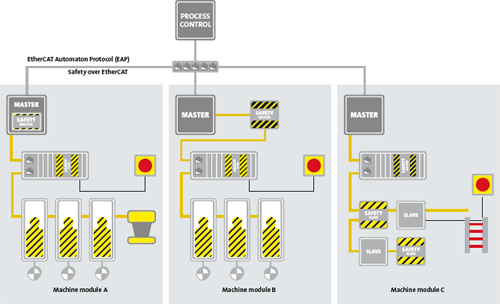
\includegraphics[width=0.8\textwidth]{fsoe_eap.png}
	\caption{EtherCAT factory-wide communication of safety-critical information \cite{technology:fsoe}}
	\label{fig:fsoe-eap}
\end{figure}
